% ------------------------------------------------------------%
% 2015-2021 - Emerson Ribeiro de Mello <mello@ifsc.edu.br>
% ------------------------------------------------------------%
% Sets aspect ratio to 4:3, and frame size to 128 mm by 96 mm
\documentclass[aspectratio=169]{beamer}
% Sets aspect ratio to 16:9, and frame size to 160 mm by 90 mm.
% \documentclass[aspectratio=169]{beamer}
% Sets aspect ratio to 16:10, and frame size to 160 mm by 100 mm.
% \documentclass[aspectratio=1610]{beamer}
\usepackage[dvipsnames]{xcolor}
\usepackage{colortbl}
\usepackage{makecell}

\definecolor{DarkCyan}{HTML}{119DA4}
\definecolor{Asparagus}{HTML}{6DA34D}
\definecolor{CambridgeBlue}{HTML}{8FBC94}
\definecolor{TeaGreen}{HTML}{C5E99B}
\definecolor{Saphire}{HTML}{4059AD}



% -------------------------------------------------%
%  Package options
% -------------------------------------------------%
%  002625, EEE5E9, 0D1821, ADF7B6, B6C454
% textbgcolor   - frametitle background color. default: 0d4f4d
% textfgcolor   - frametitle foreground color. default: ffffff
% slidebgcolor  - slide background color. default: eef1ec
% slidefgcolor  - slide text foreground color. default: 000000
% authorfgcolor - author, institute and date color. default: 000000
% itemsep - space between items (itemize, enumerate). default: 7pt
\usepackage[textbgcolor=344966,textfgcolor=ffffff,slidebgcolor=EEE5E9,itemsep=7pt]{../0-ifscyan-modelo/beamerthemeifscyan}
% -------------------------------------------------%

% A good place to get some colors
% https://material.io/resources/color/#!/?view.left=0&view.right=0&primary.color=0d4f4d
% cyan: #0D4F4D, light: #417b79,  dark: #002625
% IFSC green: normal: #32A041, light: #69d26f, dark: #007013
% IFSC red: normal: #C8191E, light: #ff5747, dark: #8f0000 
% Other colors for textbgcolor
% purple 4527a0, blue 0d47a1, grey 546e7a, redwine 880e4f, brown 6d4c41, yelllow (bg=#fbc02d, fg=000000)

% Logo
\pgfdeclareimage[height=.3\paperheight]{ifpilogo}{../0-ifscyan-modelo/figs/Logo-IFPI-Vertical.png}

\AtBeginSection[]{
  \begin{frame}
  \vfill
  \centering
  \begin{beamercolorbox}[sep=8pt,center,shadow=true,rounded=true]{title}
    \usebeamerfont{title}\insertsectionhead\par%
  \end{beamercolorbox}
  \vfill
  \end{frame}
}

% -------------------------------------------------%
%              Título 
% -------------------------------------------------%
\title{Matemática Computacional}
\subtitle{Lógica Formal}
\author{Prof. Rogério Figueredo de Sousa}
\institute{%
\href{rogerio.sousa@ifpi.edu.br}{rogerio.sousa@ifpi.edu.br}%
}%
\date{21/03/2024}
% -------------------------------------------------%

% -------------------------------------------------%
%  Início do documento 
% -------------------------------------------------%
\begin{document}

\begin{frame}[plain]
    \titlepage
\end{frame}

%\begin{frame}[plain, noframenumbering]{Licenciamento}
%    \licenciamentoLivre
%\end{frame}

%\begin{frame}[plain, noframenumbering]{Sumário}
%   \tableofcontents
%\end{frame}


\jsonp
\lstset{
    numbers=none,
    escapeinside={\%*}{*)},
}
%1
\begin{frame}{Implicação}
    As proposições podem ser combinadas na forma "\textbf{se} proposição 1, \textbf{então} proposição 2"
    \begin{itemize}
        \item Essa proposição composta é denotada por $\rightarrow$
        \item Seja proposição 1 dada por A e proposição 2 dada por B,
              reescrevemos $A \rightarrow B$, onde A é o \textbf{antecedente} e
              B é o \textbf{consequente}.
        \item Esse conectivo lógico leva o nome de \textbf{implicação} ou \textbf{condicional}.
    \end{itemize}
\end{frame}


%3
\begin{frame}{Implicação}
    \begin{itemize}
        \item Por convenção, $A \rightarrow B$ é verdadeira se A for falsa, independentemente do valor lógico de B.
    \end{itemize}

    \vspace{4mm}

    Exemplo: \textbf{Se} Fulano foi até a loja de esportes \textbf{então} foi
    até a casa de sua avó.
\end{frame}

%4
\begin{frame}{Implicação}
    \begin{itemize}
        \item \textbf{Tabela-Verdade}
    \end{itemize}

    \vspace{4mm}

    \begin{table}[hb]
        \resizebox{0.3\textwidth}{!}{
            \begin{tabular}{|c|c|c|}
                \hline
                \rowcolor{Asparagus}
                A & B & $ A \rightarrow B $ \\
                \hline
                \hline
                \rowcolor{CambridgeBlue}
                V & V & V                   \\
                \hline
                \rowcolor{TeaGreen}
                V & F & F                   \\
                \hline
                \rowcolor{CambridgeBlue}
                F & V & V                   \\
                \hline
                \rowcolor{TeaGreen}
                F & F & V                   \\
                \hline
            \end{tabular}
        }%
    \end{table}
\end{frame}

%5
\begin{frame}{Bicondicional}
    As proposições podem ser combinadas na forma "proposição 1 \textbf{se, e somente se},
    proposição 2"
    \begin{itemize}
        \item Essa proposição composta é denotada por $\leftrightarrow$
        \item Seja proposição 1 dada por A e proposição 2 dada por B, reescrevemos $A \leftrightarrow B$
        \item Esse conectivo lógico leva o nome de \textbf{Bicondicional}
        \item É uma abreviação de $(A \rightarrow B) \wedge (B \rightarrow A)$.
    \end{itemize}
\end{frame}


%6
\begin{frame}{Bicondicional}
    \textbf{Tabela-Verdade}
    \begin{table}[hb]
        \resizebox{0.7\textwidth}{!}{
            \begin{tabular}{|c|c|c|c|c|}
                \hline
                \rowcolor{Asparagus}
                A & B & $ A \rightarrow B $ & $ A \rightarrow B $ & $(A \rightarrow B) \wedge (B \rightarrow A)$ \\
                \hline
                \hline
                \rowcolor{CambridgeBlue}
                V & V & V                   & V                   & V                                            \\
                \hline
                \rowcolor{TeaGreen}
                V & F & F                   & V                   & F                                            \\
                \hline
                \rowcolor{CambridgeBlue}
                F & V & V                   & F                   & F                                            \\
                \hline
                \rowcolor{TeaGreen}
                F & F & V                   & V                   & V                                            \\
                \hline
            \end{tabular}
        }%
    \end{table}
\end{frame}

%7
\begin{frame}{Precedência de Operadores}
    Para construir uma tabela-verdade, será necessário resolver todas as possíveis
    combinações de valores lógicos das proposições existentes;
    \vspace{2mm}

    A resolução de um sistema formal deve seguir uma ordem,
    assim como acontece nas equações matemáticas:

    \begin{enumerate}
        \item $()$, $\{ \}$
        \item '
        \item  $\vee$, $\wedge$, $\oplus$
        \item $\rightarrow$
        \item $\leftrightarrow$
    \end{enumerate}
\end{frame}

%7
\begin{frame}{Precedência de Operadores}
    \begin{enumerate}
        \item $()$, $\{ \}$
        \item '
        \item  $\vee$, $\wedge$, $\oplus$
        \item $\rightarrow$
        \item $\leftrightarrow$
    \end{enumerate}

    \begin{table}[hb]
        %\resizebox{0.4\textwidth}{!}{
        \begin{tabular}{|c|c|c}
            \hline
            \rowcolor{Asparagus}
            Equação Original                               & \textcolor{LimeGreen}{Certo}                       & \textcolor{BrickRed}{Errado}                       \\
            \hline
            \hline
            \rowcolor{CambridgeBlue}
            $ A' \vee B $                                  & $ (A)' \vee B $                                    & $ (A \vee B)' $                                    \\
            \hline
            \rowcolor{TeaGreen}
            $ A \vee B \rightarrow C $                     & $ (A \vee B) \rightarrow C $                       & $ A \vee (B \rightarrow C) $                       \\
            \hline
            \rowcolor{CambridgeBlue}
            $ A \wedge B \rightarrow C \leftrightarrow D $ & $ ((A \wedge B) \rightarrow C) \leftrightarrow D $ & $ A \wedge (B \rightarrow (C \leftrightarrow D)) $ \\
            \hline
        \end{tabular}
        %    }%
    \end{table}

\end{frame}

\begin{frame}{Expressões em Português}
    \begin{center}
        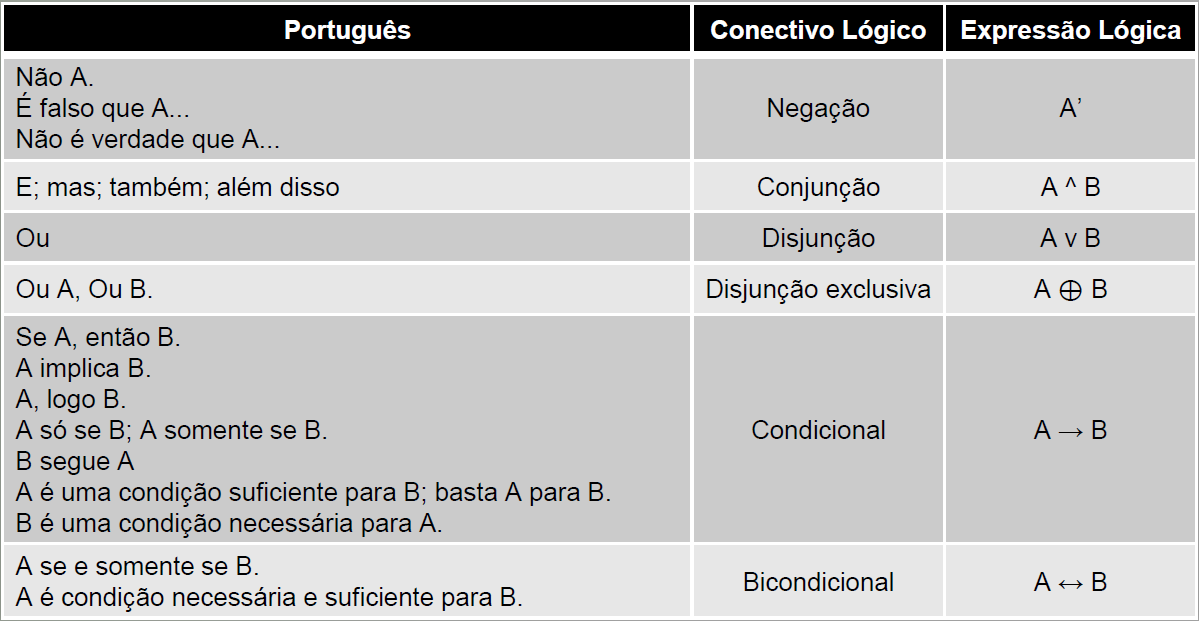
\includegraphics[width=.8\linewidth]{figs/tabelaExpressoes.png}
    \end{center}
\end{frame}

\begin{frame}{Exemplos}
    "O fogo é uma condição necessaria para a fumaça".
    \vspace{1cm}

    \textbf{De que outra maneira podemos escrever?}
    \vspace{1cm}

    "Se houver fumaça, então haverá fogo."
    \vspace{1.5cm}

    \textbf{Antecedente e consequente?}

\end{frame}

\begin{frame}{Negações corretas e incorretas}

    \begin{center}
        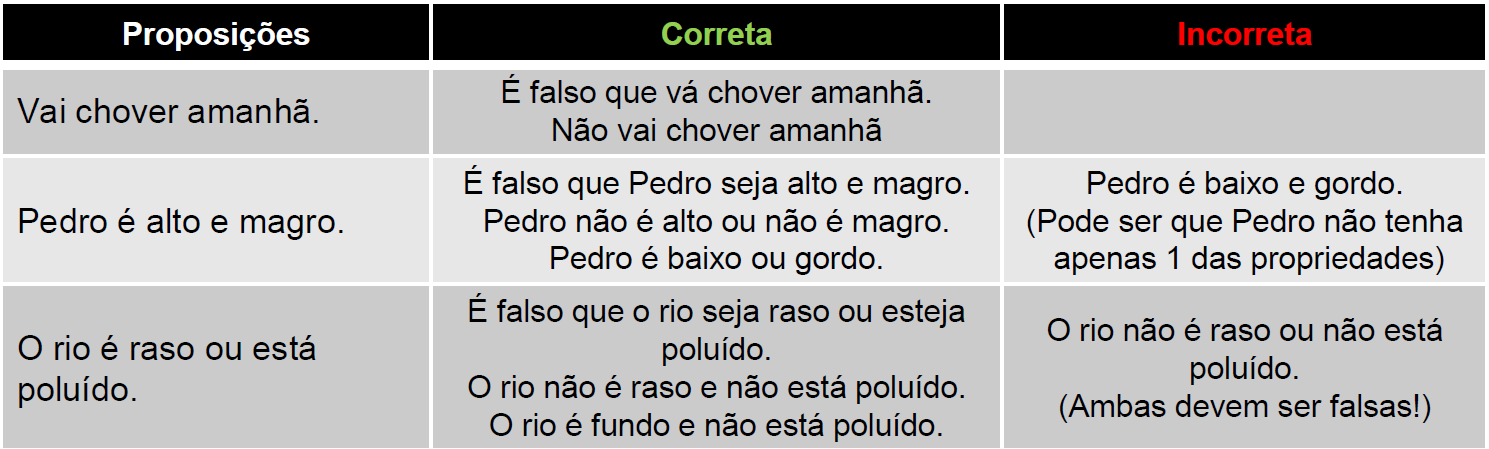
\includegraphics[width=.8\linewidth]{figs/tabelanegacoes.png}
    \end{center}

\end{frame}

\begin{frame}{Negação}
    Quais das proposições a seguir representa $P'$ se P é a proposição: "Júlia gosta de manteiga, mas detesta creme"?
    \vspace{5mm}
    \begin{enumerate}[A]
        \item Júlia detesta manteiga e creme;
        \item Júlia não gosta de manteiga nem de creme;
        \item Júlia não gosta de manteiga mas adora creme;
        \item Júlia não gosta de manteiga ou adora creme.
    \end{enumerate}

    \vspace{5mm}

    Faça a tabela-verdade.
\end{frame}


\begin{frame}{Fórmula Bem Formulada}
    Uma cadeia, no qual obedece as regras de sintaxe, como

    \[(A \rightarrow B) \wedge (B \rightarrow A)\]


    é denominada uma \textbf{fórmula bem formulada (fbf)}.

    \vspace{5mm}

    Exemplo de fórmula mal formulada,

    \[((A' \rightarrow BC \]

    Letras maiúsculas do final do alfabeto (P,Q,R,S,...) serão utilizadas para representar fbf's.

    Exemplo: $ ((A \wedge B)\wedge C) \rightarrow (B \vee C')$ pode ser representada por

    \[ P \rightarrow Q \]

\end{frame}

\begin{frame}{Exercícios}
    \begin{enumerate}
        \item Faça a tabela-verdade para cada uma das fbf:
              \begin{enumerate}[a]
                  \item $ A \vee B' \rightarrow (A \vee B)' $
                  \item $ (A \rightarrow B) \leftrightarrow (B \wedge B') $
                  \item $ (A \vee A') \rightarrow (B \wedge B')$
                  \item $ [(A \wedge B') \rightarrow C']'$
                  \item $ (A \rightarrow B) \leftrightarrow (B' \rightarrow A') $
              \end{enumerate}
    \end{enumerate}

\end{frame}

\begin{frame}{Tautologia}
    Uma fbf como a do item E), que assume apenas o valor V, é denominada \textbf{tautologia}.
    \vspace{5mm}

    Ou seja, é \textbf{verdadeira} independentemente dos valores lógicos atribuídos às proposições.
    \vspace{5mm}

    Exemplo: $ A \vee A'$
    \vspace{5mm}

    "Hoje vai ter sol ou hoje não vai ter sol".
\end{frame}

%16
\begin{frame}{Tautologia}
    É dito tautológico todo sistema lógico cuja tabela-verdade resulta apenas em valores Verdadeiros:

    $A \wedge B \leftrightarrow B \wedge A: $ (comutatividade)

    \begin{table}[hb]
        \resizebox{0.5\textwidth}{!}{
            \begin{tabular}{|c|c|c|c|c|}
                \hline
                \rowcolor{Asparagus}
                A & B & $ A \wedge B $ & $ B \wedge A $ & $ \leftrightarrow$ \\
                \hline
                \hline
                \rowcolor{CambridgeBlue}
                V & V & V              & V              & V                  \\
                \hline
                \rowcolor{TeaGreen}
                V & F & F              & F              & V                  \\
                \hline
                \rowcolor{CambridgeBlue}
                F & V & F              & F              & V                  \\
                \hline
                \rowcolor{TeaGreen}
                F & F & F              & F              & V                  \\
                \hline
            \end{tabular}
        }%
    \end{table}

\end{frame}

\begin{frame}{Contradição}
    Uma fbf como a do item C), cujo valor lógico é sempre falso, é denominada \textbf{contradição}.
    \vspace{5mm}

    Ou seja, é \textbf{falsa} independentemente dos valores lógicos atribuídos às proposições.
    \vspace{5mm}

    Exemplo: $ A \wedge A' $
    \vspace{5mm}

    “Hoje é terça-feira e hoje não é terça-feira”.

\end{frame}

\begin{frame}{Contradição}
    É dita contradição todo sistema lógico cuja tabela-verdade resulta apenas em valores Falsos:

    $(A \rightarrow B) \wedge (A \wedge B')$

    \vspace{5mm}
    \begin{table}[hb]
        \resizebox{0.7\textwidth}{!}{
            \begin{tabular}{|c|c|c|c|c|}
                \hline
                \rowcolor{Asparagus}
                A & B & $ A \rightarrow B $ & $ A \wedge B' $ & $ (A \rightarrow B) \wedge (A \wedge B') $ \\
                \hline
                \hline
                \rowcolor{CambridgeBlue}
                V & V & V                   & F               & F                                          \\
                \hline
                \rowcolor{TeaGreen}
                V & F & F                   & V               & F                                          \\
                \hline
                \rowcolor{CambridgeBlue}
                F & V & V                   & F               & F                                          \\
                \hline
                \rowcolor{TeaGreen}
                F & F & V                   & F               & F                                          \\
                \hline
            \end{tabular}
        }%
    \end{table}
\end{frame}

\begin{frame}{Contingências}
    Todo e qualquer sistema lógico que não seja Tautologia ou Contradição, será considerado contingência.

\end{frame}

% 20
\begin{frame}{Equivalência}
    Seja P e Q duas fbf's e suponha que a fbf $P \leftrightarrow Q$ seja uma tautologia.
    Se fizermos uma tabela-verdade observamos que os valores lógicos de P e Q seriam iguais em todas as linhas.
    \vspace{5mm}

    Exemplo:
    \begin{itemize}
        \item P: $ A \vee B $
        \item Q: $ B \vee A $
    \end{itemize}

    \begin{table}[hb]
        %\resizebox{0.3\textwidth}{!}{
        \begin{tabular}{|c|c|c|c|c|}
            \hline
            \rowcolor{Asparagus}
            A & B & $ A \vee B $ & $ B \vee A $ & $ P \leftrightarrow Q $ \\
            \hline
            \hline
            \rowcolor{CambridgeBlue}
            V & V & V            & V            & V                       \\
            \hline
            \rowcolor{TeaGreen}
            V & F & V            & V            & V                       \\
            \hline
            \rowcolor{CambridgeBlue}
            F & V & V            & V            & V                       \\
            \hline
            \rowcolor{TeaGreen}
            F & F & F            & F            & V                       \\
            \hline
        \end{tabular}
        % }%
    \end{table}

\end{frame}

\begin{frame}{Equivalência}
    Então, dizemos que P e Q são \textbf{equivalentes}, denotamos por $P \iff Q$.
    \vspace{5mm}

    Ou seja, $P \iff Q$ se, e somente se, $P \leftrightarrow Q$ é uma tautologia.
    \vspace{5mm}

    Logo, o item 1-E) é uma equivalência, segue

    \[(A \rightarrow B) \iff (B' \rightarrow A') \]

    \vspace{5mm}
    Quando uma fbf é equivalente a outra, elas podem ser substituídas uma pela outra.

\end{frame}

\begin{frame}{Algumas Equivalências Tautológicas}
    \begin{itemize}
        \item Comutatividade:
    \end{itemize}
    \[ A \vee B \iff B \vee A \]
    \[ A \wedge B \iff B \wedge A \]

    \begin{itemize}
        \item Associatividade:
    \end{itemize}
    \[(A \vee B) \vee C \iff A \vee (B \vee C) \]
    \[(A \wedge B) \wedge C \iff A \wedge (B \wedge C) \]

    \begin{itemize}
        \item Distributividade:
    \end{itemize}
    \[A \vee (B \wedge C) \iff (A \vee B) \wedge (A \vee C) \]
    \[A \wedge (B \vee C) \iff (A \wedge B) \vee (A \wedge C) \]

    \begin{itemize}
        \item Elementos neutros:
    \end{itemize}
    \[A \vee 0 \iff A \]
    \[A \wedge 1 \iff A \]

\end{frame}

\begin{frame}{Algumas Equivalências Tautológicas}
    Tabela-verdade elemento neutro B):

    \begin{table}[hb]
        %\resizebox{0.3\textwidth}{!}{
        \begin{tabular}{|c|c|c|c|}
            \hline
            \rowcolor{Asparagus}
            A & 1 & $ A \wedge 1 $ & $A \wedge 1 \rightarrow A $ \\
            \hline
            \hline
            \rowcolor{CambridgeBlue}
            V & V & V              & V                           \\
            \hline
            \rowcolor{TeaGreen}
            F & V & F              & V                           \\
            \hline
        \end{tabular}
        % }%
    \end{table}

    \begin{itemize}
        \item Complementares
    \end{itemize}
    \[A \vee A' \iff 1 \]
    \[A \wedge A' \iff 0 \]

\end{frame}

\begin{frame}{Leis de \textit{De Morgan}}
    O matemático inglês Augusto De Morgan (1806 - 1871) foi o primeiro a enunciar algumas equivalências lógicas
    (e de conjuntos). Estas equivalências convertem operações lógicas E em OU e vice-versa e são amplamente utilizadas
    na construção de sistemas lógicos:

    \textbf{\[ (A \vee B)' \iff A' \wedge B' \]}

    \vspace{5mm}

    \textbf{\[ (A \wedge B)' \iff A' \vee B' \]}

\end{frame}

\begin{frame}{Leis de \textit{De Morgan}}
    Na prática, não importa o número de proposições. Ex.:

    \vspace{5mm}

    \textbf{\[ (A \vee B \vee C \vee D)' \iff A' \wedge B' \wedge C' \wedge D' \]}

    \vspace{5mm}

    \textbf{\[ (A \wedge B \wedge C \wedge D \wedge E)' \iff A' \vee B' \vee C' \vee D' \vee E' \]}

\end{frame}

\begin{frame}{Regras de Equivalência}

    \begin{center}
        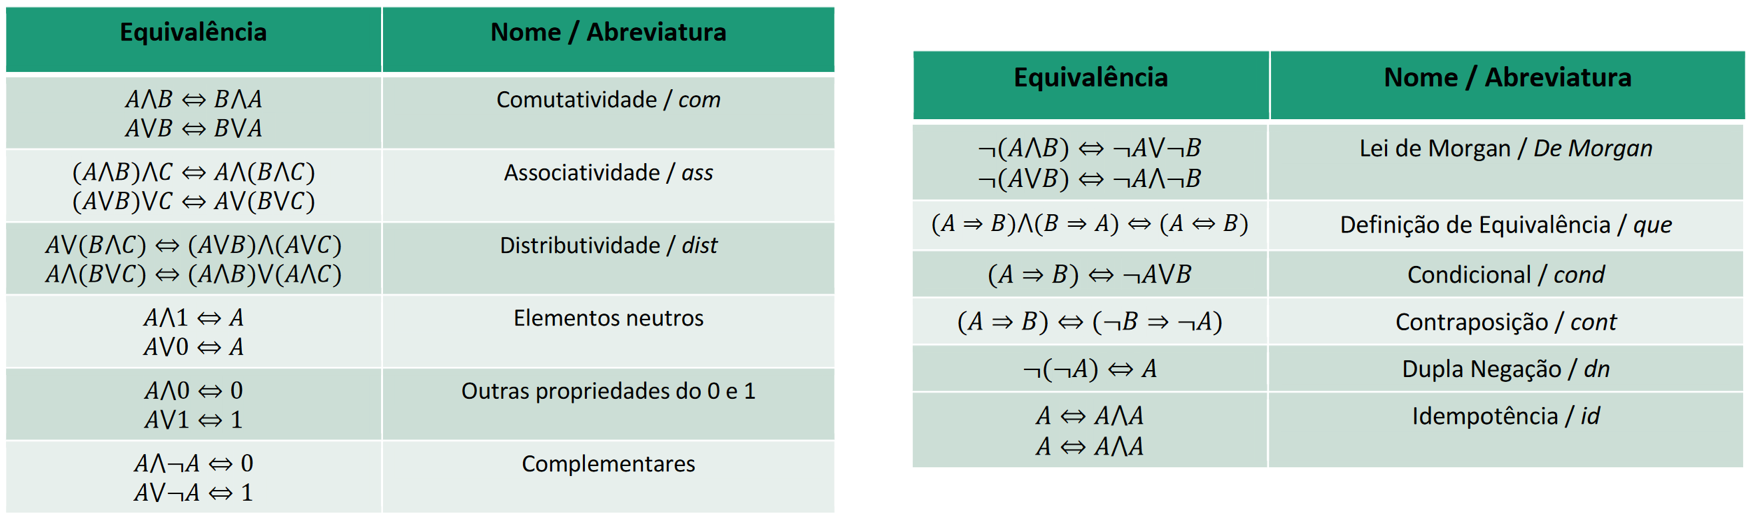
\includegraphics[width=.9\linewidth]{figs/equivalencias.png}
    \end{center}

\end{frame}

\begin{frame}{Questões Poscomp (1/7)}
    \textbf{Poscomp[2013, q11]}: Considere as sentenças a seguir:

    \textbf{P}: Pedro faz as tarefas todos os dias.

    \textbf{Q}: Pedro terá boas notas no final do ano.

    \begin{itemize}
        \item Assinale a alternativa que apresenta, corretamente, a tradução em linguagem simbólica da negação da sentença composta a seguir:
        \item “Se Pedro faz as tarefas todos os dias, então Pedro terá boas notas no final do ano.”
              \begin{enumerate}
                  \item $P \rightarrow Q $
                  \item $ P \leftrightarrow Q $
                  \item $ P \wedge \sim Q$
                  \item $\sim P \wedge \sim Q$
                  \item $\sim P \wedge Q $
              \end{enumerate}
    \end{itemize}

\end{frame}

\begin{frame}{Questões Poscomp (2/7)}

    \textbf{Poscomp[2013, q13]}: Admita que um novo conectivo binário, rotulado pelo símbolo $\updownarrow$, seja definido
    pela tabela-verdade ao lado. Com base nessa definição e nas operações usuais com os conectivos $\vee$, $\wedge$ e $\sim$,
    considere as afirmativas a seguir.

    \begin{columns}
        \begin{column}{0.6\textwidth}
            \begin{enumerate}[I]
                \item $P \updownarrow Q$ é equivalente a $Q \updownarrow P$
                \item $(P \updownarrow Q) \vee (Q \updownarrow P)$ não é uma contingência.
                \item  $(Q \updownarrow P) \wedge (P \updownarrow Q)$ é uma contradição.
                \item  $\sim [(Q \updownarrow P) \wedge (P \updownarrow Q)]$ é uma tautologia.
            \end{enumerate}

            Assinale a alternativa correta.
            \begin{enumerate}[a]
                \item Somente as afirmativas I e II são corretas.
                \item Somente as afirmativas I e IV são corretas.
                \item Somente as afirmativas III e IV são corretas.
                \item Somente as afirmativas I, II e III são corretas.
                \item Somente as afirmativas II, III e IV são corretas.
            \end{enumerate}
        \end{column}
        \begin{column}{0.4\textwidth}  %%<--- here
            \begin{center}
                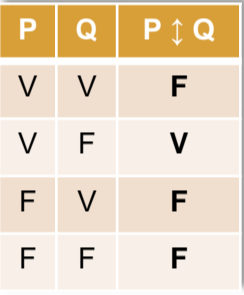
\includegraphics[width=.4\linewidth]{figs/tabelaposcomp.png}
            \end{center}
        \end{column}
    \end{columns}

\end{frame}

\begin{frame}{Questões Poscomp (3/7)}

    Assinale a proposição logicamente equivalente a
    $\lnot(p \vee q) \vee (\lnot p \wedge q)$

    \begin{enumerate}[a]
        \item $ \lnot p \wedge (q \vee \lnot q) $
        \item $ \lnot p$
        \item $ (p \vee q) \wedge (p \vee \lnot q)$
        \item $ (p \vee q) \vee (p \wedge \lnot q)$
        \item $ p $
    \end{enumerate}

\end{frame}

\begin{frame}{Questões Poscomp (4/7)}

    Considere as seguintes proposições:

    \begin{enumerate}[I]
        \item $ \lnot p \vee q$
        \item $ \lnot(p \wedge \lnot q)$
        \item $ p \rightarrow q$
        \item $(V \rightarrow q) \vee (p \rightarrow F) $
    \end{enumerate}

    Quais as proposições acima são logicamente equivalentes?

    \begin{enumerate}[a]
        \item Somente I $\equiv$ III
        \item Somente I $\equiv$ II
        \item Somente I $\equiv$ II $\equiv$ III
        \item I $\equiv$ III e II $\equiv$ III mas III $\not\equiv$ IV
        \item I, II, III, IV são todas equivalentes.
    \end{enumerate}

\end{frame}

\begin{frame}{Questões Poscomp (5/7)}

    A sentença lógica $ A \wedge (B \vee \lnot C )$ é equivalente a

    \begin{enumerate}[A]
        \item $ A \wedge (\lnot B \wedge C) $
        \item $ \lnot A \vee \lnot (B \vee \lnot C)$
        \item $ \lnot A \vee (\lnot B \wedge C)$
        \item Todas as respostas anteriores
        \item Nenhuma das respostas anteriores
    \end{enumerate}

\end{frame}

\begin{frame}{Questões Poscomp (6/7)}

    Existem três suspeitos de invadir uma rede de computadores: André, Bruna e Carlos.
    Sabe-se que a invasão foi efetivamente cometida por um ou por mais de um deles,
    já que podem ter agido individualmente ou não. Sabe-se, ainda, que:

    \begin{enumerate}[I]
        \item Se André é inocente, então Bruna é culpada.
        \item Ou Carlos é culpado ou Bruna é culpada, mas não os dois.
        \item Carlos não é inocente.
    \end{enumerate}

    Com base nestas considerações, conclui-se que:

    \begin{enumerate}[A]
        \item Somente André é inocente.
        \item Somente Bruna é culpada.
        \item Somente Carlos é culpado.
        \item São culpados apenas Bruna e Carlos.
        \item São culpados apenas André e Carlos.
    \end{enumerate}

\end{frame}


\begin{frame}{Questões Poscomp (7/7)}

    Os conectores lógicos $\vee$, $\rightarrow$ são lidos como ``ou'' e "implica".
    O operador ``não'' ~é representado por $\lnot$. Considerando esta notação,
    a tabela verdade da proposição $ (P \rightarrow Q) \rightarrow (\lnot Q \vee P)$,
    assumindo que a sequencia de valores de \textit{P} é \{V,V,F,F\} e a de \textit{Q} é \{V,F,V,F\},
    tem os valores:

    \begin{enumerate}[a]
        \item \{ F,F,F,F \}
        \item \{ V,V,V,V \}
        \item \{ V,V,F,V \}
        \item \{ F,F,V,V \}
        \item \{ V,F,V,F \}
    \end{enumerate}


\end{frame}

\section{Lógica Proposicional}
\begin{frame}{Argumentos Válidos}
    Um argumento pode ser representado em forma simbólica como
    \[ P_1 \wedge P_2 \wedge P_3 \wedge ... \wedge P_n \rightarrow Q \]

    Onde $P_1$, $P_2$, $P_3$ … são proposições dadas, chamadas de \textbf{hipóteses} do argumento,
    e $Q$ é a \textbf{conclusão}.

    \vspace{5mm}
    Em geral, $P_i$ e $Q$ representam fbf's.

    \vspace{5mm}
    Quando que deve ser considerado um \underline{argumento válido}?

\end{frame}


\begin{frame}{Argumentos Válidos}
    \underline{Quando deve ser considerado um argumento válido?}
    \vspace{5mm}

    $Q$ é uma conclusão lógica de $P_1$, $...$ , $P_n$ sempre que a
    verdade das proposições $P_1, ... , P_n$ implica na verdade de $Q$.
    \vspace{5mm}

    Considere o argumento (contra-exemplo):

    ``Luis Inácio é o presidente do Brasil. Florianópolis é a capital de Santa Catarina.
    Portanto, o dia tem 24 horas''.

    \[ A \wedge B \rightarrow C \]

    Duas hipóteses e a conclusão, mas nesse caso \textbf{não} consideramos o argumento válido,
    pois a conclusão é um fato verdadeiro isolado das hipóteses.


\end{frame}

\begin{frame}{Argumentos Válidos}
    Um argumento válido deveria ser intrinsicamente verdadeiro, sendo assim,
    segue definição.
    \vspace{5mm}

    Definição: A fbf proposicional

    \[ P_1 \wedge P_2 \wedge P_3 \wedge ... \wedge P_n \rightarrow Q \]

    é um \textbf{argumento válido} quando for uma tautologia.
    \vspace{5mm}

    \textit{Obs: no último exemplo o argumento $(A \wedge B \rightarrow C)$ não é uma tautologia,
        por isso não era um argumento válido}.

\end{frame}

\begin{frame}{Argumentos Válidos}
    Exemplo 1)

    ``Se Luis Inácio for presidente do Brasil, então Geraldo Alckmin é o vice-presidente.
    Luis Inácio é presidente do Brasil. Portanto, Geraldo Alckmin é o vice-presidente do Brasil''.
    \vspace{5mm}

    Duas hipóteses:
    \begin{enumerate}
        \item Se \textcolor{red}{Luis Inácio for presidente do Brasil}, então \textcolor{ForestGreen}{Geraldo Alckmin é o vice-presidente}
        \item \textcolor{red}{Luis Inácio é presidente do Brasil}.
    \end{enumerate}

    Conclusão:

    \textcolor{ForestGreen}{Geraldo Alckmin é o vice-presidente do Brasil}.

    \vspace{3mm}
    \textbf{Representação simbólica:} $A \rightarrow B \wedge A \rightarrow B$, que é uma tautologia.


\end{frame}

%38
\begin{frame}{Ex. 2: Validade de Argumentos}
    \textbf{Argumento:} $P_1 \wedge P_2 \rightarrow Q$

    $P_1$: ``Se está chovendo, então há nuvens.''

    \underline{$P_2$: ``Está chovendo.''}

    $Q$: ``Há nuvens.''

    \vspace{3mm}
    \textbf{Proposições:}

    A: Está chovendo.

    B: Há nuvens
    \vspace{3mm}

    \textbf{Dedução/validação:}

    $P_1$: $A \rightarrow B$

    \underline{$P_2$: A}

    Q: B
    \vspace{4mm}

    \textit{\textbf{Dedução Válida?}}


\end{frame}

%39
\begin{frame}{Ex. 3: Validade de Argumentos}
    \textbf{Argumento:} $P_1 \wedge P_2 \rightarrow Q$

    $P_1$: ``Se está chovendo, então há nuvens.''

    \underline{$P_2$: ``Há Nuvens.''}

    $Q$: ``Está chovendo.''

    \vspace{3mm}
    \textbf{Proposições:}

    A: Está chovendo.

    B: Há nuvens
    \vspace{3mm}

    \textbf{Dedução/validação:}

    $P_1$: $A \rightarrow B$

    \underline{$P_2$: B}

    Q: A
    \vspace{4mm}

    \textit{\textbf{Dedução Válida?}}


\end{frame}

\begin{frame}{Regras de Dedução}
    Sequência de demonstração:
    \vspace*{4mm}

    \textbf{Hipóteses: $P_1$, $P_2$, ... , $P_n$}
    \vspace*{2mm}

    \textbf{Fbf's: fbf1, fbf2,..}
    \vspace*{2mm}

    \textbf{Conclusão: Q.}

\end{frame}

\begin{frame}{Lógica Proposicional}
    Existem, basicamente, dois tipos de regra de dedução: \textbf{equivalências e inferências}.
    \vspace*{4mm}

    \begin{block}{Equivalências}
        Permitem que as fbf's sejam reescritas mantendo o valor lógico.
    \end{block}

    \vspace*{4mm}

    \begin{block}{Inferências}
        Permitem a dedução de novas fbf's a partir de fbf's anteriores.
    \end{block}


\end{frame}

\begin{frame}{Regras de Equivalência}

    \begin{center}
        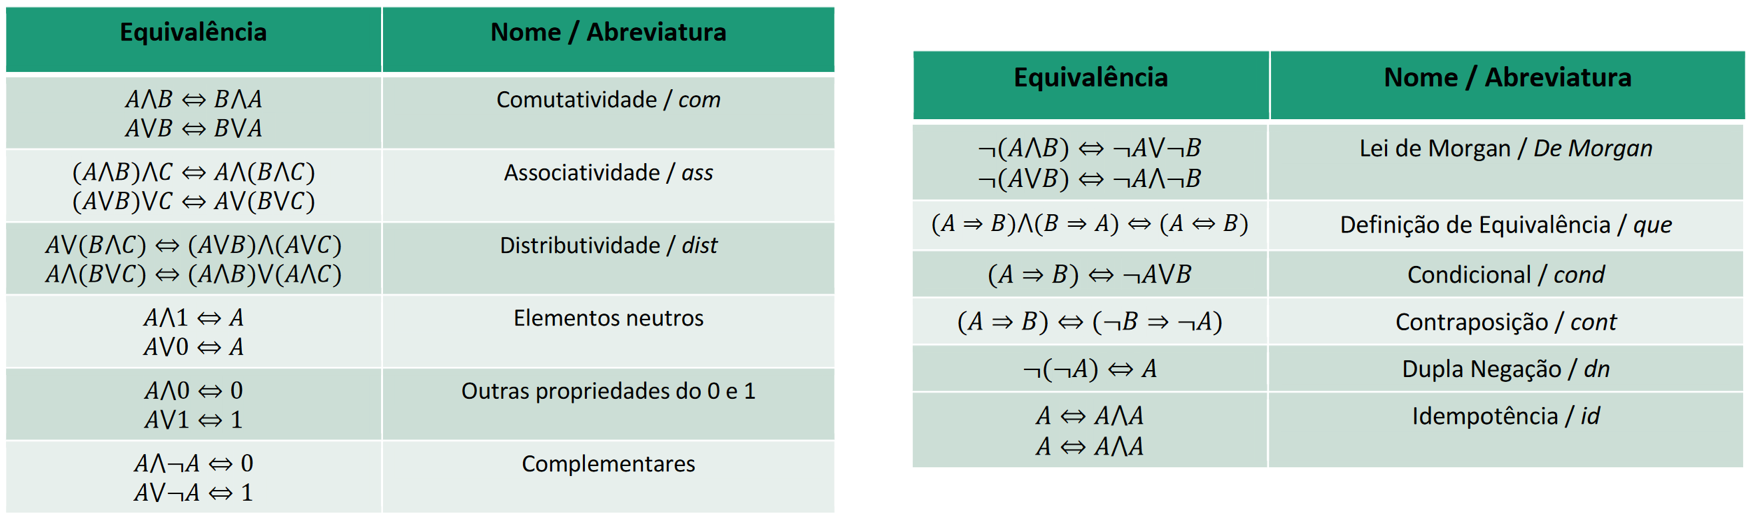
\includegraphics[width=.9\linewidth]{figs/equivalencias.png}
    \end{center}

\end{frame}

\begin{frame}{Regras de Equivalência}
    Exemplo: suponha o argumento proposicional

    \[ (A' \vee B') \vee C \]

    então uma sequência de demonstração ficaria,
    \vspace{2mm}

    \begin{itemize}
        \item $ (A' \vee B') \vee C $   (hipótese)
        \item $ (A \wedge B)' \vee C $    (1, De Morgam)
        \item $ (A \wedge B) \rightarrow C $    (2, condicional)
    \end{itemize}
\end{frame}

\begin{frame}{Regras de Equivalência}
    Exemplo: Se Marcia não está com fome, então ela não vai a padaria. Além disso,
    se Márcia está com fome e vai à padaria ou não vai à padaria, então
    ela vai à padaria.

    A: Márcia vai à padaria.
    B: Márcia está com fome.

    \pause

    \[ (B' \rightarrow A') \wedge (B \wedge (A \vee A') \rightarrow A)\]
    \pause

    \textbf{(Complementares) $ A \vee A' \leftrightarrow 1$}:

    $(B' \rightarrow A') \wedge (B \wedge (1) \rightarrow A)$
    \pause

    \textbf{Contraposição $ (A \rightarrow B) \leftrightarrow (B' \rightarrow A')$ e Elemento Neutro: $A \wedge 1 \leftrightarrow A$}:

    $(A \rightarrow B) \wedge (B \rightarrow A)$
    \pause

    \textbf{Definição de Equivalência: $ (A \rightarrow B) \wedge (B \rightarrow A) \leftrightarrow (A \leftrightarrow B)$}:

    $ A \leftrightarrow B$
    \pause

    \vspace*{4mm}
    \textbf{Márcia vai à padaria se, e somente se ela está com fome}

\end{frame}

\begin{frame}{Regras de Inferência}
    \begin{center}
        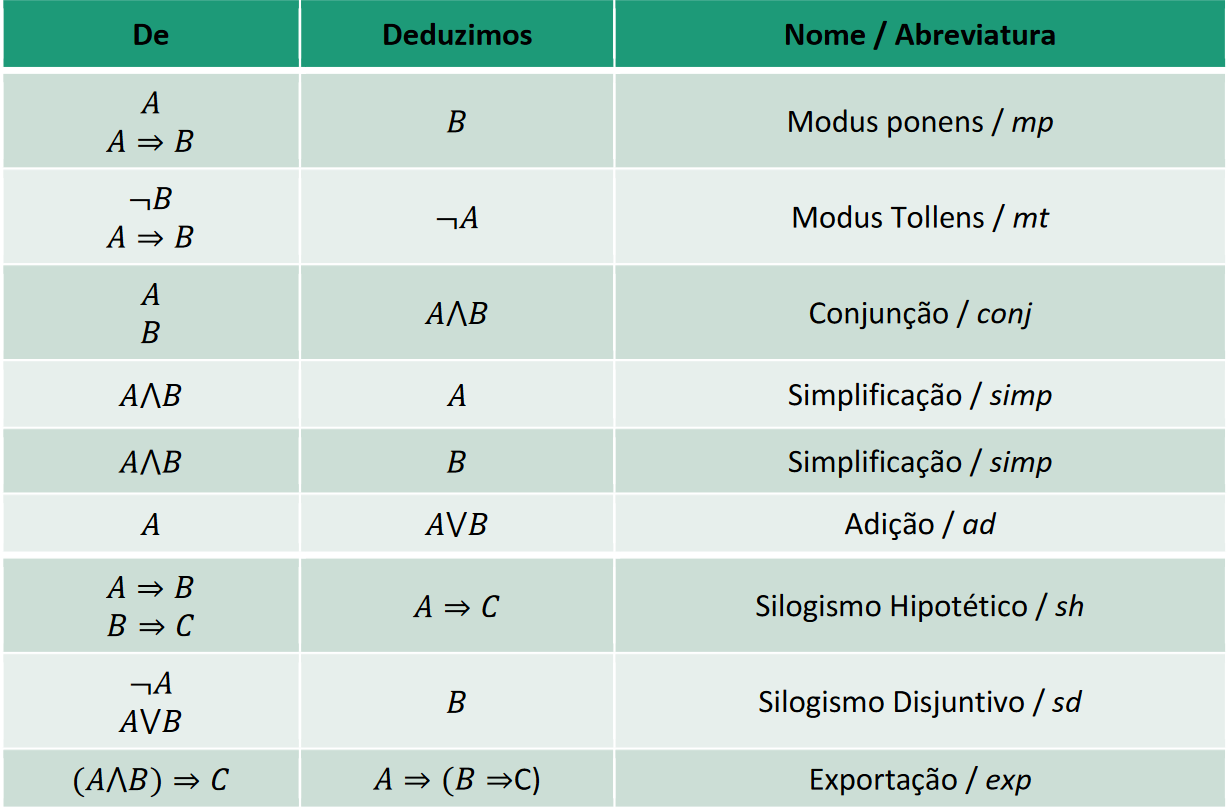
\includegraphics[width=.7\linewidth]{figs/inferencia.png}
    \end{center}
\end{frame}

%46
\begin{frame}{Regras de Inferência}
    Se uma ou mais fbf's contidas na primeira coluna das regras de inferência,
    fazem parte de uma sequência da demonstração, então podemos substituí-las
    pela fbf contida na segunda coluna.

    \vspace{3mm}
    As regras de inferência não funcionam em ambas direções.

    \textbf{Exemplo}: suponha $A \rightarrow (B \wedge C)$ e A duas hipóteses de um argumento,
    uma sequência de demonstração seria:

    \begin{itemize}
        \item $A \rightarrow (B \wedge C)$ \textbf{(hipótese)}
        \item $A$ \textbf{(hipótese)}
        \item $ B \wedge C$ \textbf{(1,2,modus ponens)}
    \end{itemize}

    Depois da última movimentação, a FBF se parece com a adição, mas não podemos inferir nem B e nem C


\end{frame}

\begin{frame}{Regras de Inferência}
    Exemplo: dê o próximo passo da demonstração e justifique.
    \vspace{4mm}

    \begin{itemize}
        \item $(A \wedge B') \rightarrow C$ \textbf{(hipótese)}
        \item $C'$ \textbf{(hipótese)}
        \item ?
    \end{itemize}
\end{frame}

\begin{frame}{Regras de Inferência}
    Exemplo: dê o próximo passo da demonstração e justifique.
    \vspace{4mm}

    \begin{itemize}
        \item $(A \wedge B') \rightarrow C$ \textbf{(hipótese)}
        \item $C'$ \textbf{(hipótese)}
        \item $ (A \wedge B')' $ \textbf{(1,2,mt)}
    \end{itemize}
\end{frame}

%49
\begin{frame}{Ex. 1: Demonstração}
    \textbf{Argumento:} $P_1 \wedge P_2 \rightarrow Q$

    $P_1$: ``Se está chovendo, então há nuvens.''

    \underline{$P_2$: ``Está chovendo.''}

    $Q$: ``Há nuvens.''

    \vspace{3mm}
    \textbf{Proposições:}

    A: Está chovendo.

    B: Há nuvens
    \vspace{3mm}

    \textbf{Dedução/validação:}

    $P_1$: $A \rightarrow B$

    \underline{$P_2$: A}

    Q: B
    \vspace{4mm}

    \textit{\textbf{Dedução Válida?}}


\end{frame}


\begin{frame}{Exemplo 1 :Demonstração}
    \[ (A \rightarrow B ) \wedge A \rightarrow B \]

    \begin{itemize}
        \item $A \rightarrow B$ \textbf{(hipótese, V)}
        \item $A$ \textbf{(hipótese, V)}
        \item $ B $ \textbf{(1,2,mp)}
    \end{itemize}
\end{frame}

\begin{frame}{Exemplo 2}
    \textbf{Argumento:} $P_1 \wedge P_2 \rightarrow Q$

    $P_1$: ``Se está chovendo, então há nuvens.''

    \underline{$P_2$: ``Está chovendo.''}

    $Q$: ``Há nuvens.''

    \vspace{3mm}
    \textbf{Proposições:}

    A: Está chovendo.

    B: Há nuvens
    \vspace{3mm}

    \textbf{Dedução/validação:}

    $P_1$: $A \rightarrow B$

    \underline{$P_2$: B}

    Q: B
    \vspace{4mm}

    \textit{\textbf{Dedução Válida? Não, não é um argumento válido.}}


\end{frame}

\begin{frame}{Exemplo de Demonstração Completa}
    Usando lógica proposicional, prove que o argumento é válido.

    \[ A \wedge (B \rightarrow C) \wedge \left[ (A \wedge B) \rightarrow (D \vee C') \right] \wedge B \rightarrow D \]

    \textbf{Exercício 1:} provar a validade de:

    \[ \left[ A \rightarrow (B \vee C) \right] \wedge B' \wedge C' \rightarrow A' \]
    \vspace{4mm}

    \textbf{Exercício 2:} provar a validade de:

    \[ A' \wedge B \wedge [B \rightarrow (A \vee C)] \rightarrow C \]

\end{frame}

\begin{frame}{Método Dedutivo}
    Suponha que o argumento que queremos provar tenha a forma

    \[ P_1 \wedge P_2 \wedge P_3 \wedge ... \wedge P_n \rightarrow (R \rightarrow S) \]

    onde a conclusão é uma implicação.


    Ao invés de usar $P_1, ... , P_n$ como hipótese e $R \rightarrow S$ de conclusão,
    o método dedutivo nos permite adicionar R como hipótese,

    \[ P_1 \wedge P_2 \wedge P_3 \wedge ... \wedge P_n \wedge R \rightarrow S \]

\end{frame}


\begin{frame}{Exemplo}
    Use lógica proposicional para provar

    \[ [A \rightarrow (A \rightarrow B)] \rightarrow (A \rightarrow B)  \]

    e

    \[ (A \rightarrow B) \wedge (B \rightarrow C) \rightarrow (A \rightarrow C) \] (silogismo hipotético)

\end{frame}


\begin{frame}{Exercícios}

    Use lógica proposicional para provar

    \begin{itemize}
        \item $(A' \vee B) \wedge (B \rightarrow C) \rightarrow (A \rightarrow C) $
        \item $ (A \rightarrow B) \wedge (C' \vee A) \wedge C \rightarrow B $
    \end{itemize}
\end{frame}

\begin{frame}{Argumentos Verbais}

    Exemplo 1: Considere o argumento “Se as taxas de juros caírem, o mercado imobiliário
    vai melhorar. A taxa federal de descontos vai cair ou o mercado imobiliário não vai
    melhorar. As taxas de juros vão cair. Portanto, a taxa federal de descontos vai cair
    \vspace{4mm}

    Resolução:

    \textbf{J:} A taxa de juros vai cair.

    \textbf{I:} O mercado imobiliário vai melhorar.

    \textbf{F:} A taxa federal de descontos vai cair.

    O argumento fica: $(J \rightarrow I) \wedge (F \vee I') \wedge J \rightarrow F$, basta \textbf{provar se o argumento é válido}.

\end{frame}

\begin{frame}{Argumentos Verbais}
    Exemplo 2: ``Meu cliente é canhoto mas, se o diário não tiver sumido, então meu
    cliente não é canhoto; portanto o diário sumiu.''
    \vspace{4mm}

    Exemplo 3: ``Se segurança é um problema, então o controle será aumentado.
    Se segurança não é um problema, então os negócios na Internet irão aumentar.
    Portanto, se o controle não for aumentado, os negócios na Internet crescerão.''

\end{frame}
\end{document}